\documentclass{beamer}
\mode<presentation>
\usepackage{amsmath}
\usepackage{amssymb}
%\usepackage{advdate}
\usepackage{adjustbox}
\usepackage{subcaption}
\usepackage{enumitem}
\usepackage{multicol}
\usepackage{mathtools}
\usepackage{listings}
\usepackage{url}
\usepackage{minted}
% \usepackage{gvv}

\usepackage{tcolorbox}
\tcbuselibrary{minted,breakable,xparse,skins}



\definecolor{bg}{gray}{0.95}
\DeclareTCBListing{mintedbox}{O{}m!O{}}{%
  breakable=true,
  listing engine=minted,
  listing only,
  minted language=#2,
  minted style=default,
  minted options={%
    linenos,
    gobble=0,
    breaklines=true,
    breakafter=,,
    fontsize=\scriptsize,
    numbersep=8pt,
    #1},
  boxsep=0pt,
  left skip=0pt,
  right skip=0pt,
  left=25pt,
  right=0pt,
  top=3pt,
  bottom=3pt,
  arc=5pt,
  leftrule=0pt,
  rightrule=0pt,
  bottomrule=2pt,
  toprule=2pt,
  colback=bg,
  colframe=orange!70,
  enhanced,
  overlay={%
    \begin{tcbclipinterior}
    \fill[orange!20!white] (frame.south west) rectangle ([xshift=20pt]frame.north west);
    \end{tcbclipinterior}},
  #3,
}


\def\UrlBreaks{\do\/\do-}
\usetheme{Madrid}
\usecolortheme{lily}
\setbeamertemplate{footline}
{
  \leavevmode%
  \hbox{%
  \begin{beamercolorbox}[wd=\paperwidth,ht=2.25ex,dp=1ex,right]{author in head/foot}%
    \insertframenumber{} / \inserttotalframenumber\hspace*{2ex} 
  \end{beamercolorbox}}%
  \vskip0pt%
}
\setbeamertemplate{navigation symbols}{}

\providecommand{\nCr}[2]{\,^{#1}C_{#2}} % nCr 
\providecommand{\nPr}[2]{\,^{#1}P_{#2}} % nPr
\providecommand{\mbf}{\mathbf}
\providecommand{\pr}[1]{\ensuremath{\Pr\left(#1\right)}}
\providecommand{\qfunc}[1]{\ensuremath{Q\left(#1\right)}}
\providecommand{\sbrak}[1]{\ensuremath{{}\left[#1\right]}}
\providecommand{\lsbrak}[1]{\ensuremath{{}\left[#1\right.}}
\providecommand{\rsbrak}[1]{\ensuremath{{}\left.#1\right]}}
\providecommand{\brak}[1]{\ensuremath{\left(#1\right)}}
\providecommand{\lbrak}[1]{\ensuremath{\left(#1\right.}}
\providecommand{\rbrak}[1]{\ensuremath{\left.#1\right)}}
\providecommand{\cbrak}[1]{\ensuremath{\left\{#1\right\}}}
\providecommand{\lcbrak}[1]{\ensuremath{\left\{#1\right.}}
\providecommand{\rcbrak}[1]{\ensuremath{\left.#1\right\}}}
\theoremstyle{remark}
\newtheorem{rem}{Remark}
\newcommand{\sgn}{\mathop{\mathrm{sgn}}}
\providecommand{\abs}[1]{\left\vert#1\right\vert}
\providecommand{\res}[1]{\Res\displaylimits_{#1}} 
\providecommand{\norm}[1]{\lVert#1\rVert}
\providecommand{\mtx}[1]{\mathbf{#1}}
\providecommand{\mean}[1]{E\left[ #1 \right]}
\providecommand{\fourier}{\overset{\mathcal{F}}{ \rightleftharpoons}}
%\providecommand{\hilbert}{\overset{\mathcal{H}}{ \rightleftharpoons}}
\providecommand{\system}{\overset{\mathcal{H}}{ \longleftrightarrow}}
	%\newcommand{\solution}[2]{\textbf{Solution:}{#1}}
%\newcommand{\solution}{\noindent \textbf{Solution: }}
\providecommand{\dec}[2]{\ensuremath{\overset{#1}{\underset{#2}{\gtrless}}}}
\newcommand{\myvec}[1]{\ensuremath{\begin{pmatrix}#1\end{pmatrix}}}
\let\vec\mathbf

\lstset{
%language=C,
frame=single, 
breaklines=true,
columns=fullflexible
}

\numberwithin{equation}{section}

\title{Presentation}
\author{Sri Sathwik Desaboina \\ AI24BTECH11007}

\date{\today} 
\begin{document}

\begin{frame}
\titlepage
\end{frame}

\section*{Outline}
\begin{frame}
\tableofcontents
\end{frame}
\section{Problem}
\begin{frame}
\frametitle{Problem Statement}
%

Show that the point $\myvec{x \\ y}$ given by $x = \frac{2at}{1 + t^2}$ and $y = \frac{a(1 - t^2)}{1 + t^2}$ lies on a circle for all real values of $t$ such that $-1 \leq t \leq 1$, where $a$ is any given real number.
\end{frame}

%\subsection{Literature}
\section{Solution}
\subsection{Usage of variables}
\begin{frame}
\frametitle{Usage of variables}
	\begin{tabular}[12pt]{ |c| c| c|}
    \hline
    \textbf{S.No} & \textbf{variables used}&\textbf{description}\\ 
    \hline
	$1$ & \textit{t} & a variable which takes the real values in the range $(-1,1)$\\
    \hline
	$2$ & \textit{a} & it is a fixed real number \\
    \hline
	$3$ & $\vec{A(t)}$ & it is a transformation matrix of parameter t\\
    \hline
	$4$ & $\vec{v(t)}$ & it represent the parameter t and allows to define x and y \\
    \hline
	$5$ & $\vec{p(t)}$ & a point with coordinates x and y. \\
    \hline
    \end{tabular}

\end{frame}
\subsection{Parametric form}
\begin{frame}
\frametitle{Parametric form}
Given $x$ and $y$ in the parametric form,\\
	\begin{align}
		x &= \frac{2at}{1 + t^2},\\
		\quad y &= \frac{a(1 - t^2)}{1 + t^2}
	\end{align}
	Let $\vec{p(t)}$ be equal to,\\
	\begin{align}
	\mathbf{p}(t) = \myvec{x \\ y} = \myvec{\frac{2at}{1 + t^2} \\ \frac{a(1 - t^2)}{1 + t^2}}.
	\end{align}


\end{frame}
\subsection{Matrix equation}
\begin{frame}
\frametitle{Matrix equation}
	The transformation matrix $\vec{A(t)}$ and $\vec{v(t)}$ with parameter $t$ are,\\
	\begin{align}
		\implies \mathbf{A}(t) & = \myvec{ \frac{2a}{1+t^2} & 0 \\ 0 & \frac{a(1-t^2)}{1+t^2}},\\ \implies \mathbf{v(t)} &= \myvec{t \\ 1},\\ \mathbf{p(t)} &= \mathbf{A(t)} \mathbf{v(t)}, \\\implies  \mathbf{p}(t) & = \myvec{ \frac{2a}{1+t^2} & 0 \\ 0 & \frac{a(1 - t^2)}{1+t^2} } \myvec{t \\ 1},\\ 
	\end{align}
\end{frame}
%\section{Plot}
\subsection{Verification}
\begin{frame}[fragile]
\frametitle{Verification}
Now, if we check the value of ,
    \begin{align}
    \mathbf{p}(t)^\top \myvec{ 1 & 0 \\ 0 & 1 } \mathbf{p}(t)
    \end{align}
	We get,\\
  \begin{align}
    \mathbf{p}(t)^\top \myvec{ 1 & 0 \\ 0 & 1 } \mathbf{p}(t)=a^2
    \end{align}

	$\implies$ We proved that the given points lie on a circle $x^2 + y^2 = a^2$.\\
	Since we have the values of $t$ in $(-1,1)$, the y-coordinate of the points is always positive.\\
	We get a semi-circle with those points.
\end{frame}

\section{Codes}
\subsection{C code to generate points}

\begin{frame}[fragile,allowframebreaks]
\frametitle{C code to generate points}
\begin{mintedbox}{c}[break at=.8\textheight]
#include <stdio.h>

int main() {
    // Declare a pointer to the file
    FILE *file;

    // Open the file points.dat for writing (will create it if it doesn't exist)
    file = fopen("points.dat", "w");

    // Check if the file was opened successfully
    if (file == NULL) {
        printf("Error opening file!\n");
        return 1;  // Return 1 if there was an error
    }

    // Write the origin point O to the file (x=0, y=0)
    fprintf(file, "0.00000 0.00000\n");

    // Define the number of points and the range of the parameter t
    int num_points = 100;  // Number of points to generate
    double t_start = -1.0, t_end = 1.0;  // Range of t (from -1 to 1)
    double t_increment = (t_end - t_start) / (num_points - 1);  // Step size for t

    // Loop to calculate points and write them to the file
    for (int i = 0; i < num_points; i++) {
        // Calculate t value for the current point
        double t = t_start + i * t_increment;

        // Parametric equations to calculate x and y
        double x = (2 * t) / (1 + t * t);  // Equation for x
        double y = (1 - t * t) / (1 + t * t);  // Equation for y

        // Write the calculated point (x, y) to the file with 5 decimal precision
        fprintf(file, "%.5f %.5f\n", x, y);
    }

    // Close the file
    fclose(file);

    // Print success message
    printf("Data written to points.dat successfully.\n");

    return 0;
}



  \end{mintedbox}
\end{frame}

  
  \subsection{Plotting the figure using Python}
\begin{frame}[fragile,allowframebreaks]
\frametitle{Plotting the figure using Python}
   \begin{mintedbox}{Python}[break at=.8\textheight]
import numpy as np
import matplotlib.pyplot as plt

# Load the points from the file (now space-separated)
data = np.loadtxt("points.dat", delimiter=" ")

# Extract the center point O from the data file (first point)
center_x = data[0, 0]  # Should be 0.0
center_y = data[0, 1]  # Should be 0.0

# Separate the circle points and transformed points
circle_points = data[1:101]  # Assuming first 100 points are from the circle
transformed_points = data[101:]  # Remaining points are transformed points

# Create a plot with minimized dimensions
plt.figure(figsize=(5, 4))  # Changed dimensions to 5x4 inches

# Plot the circle points
plt.plot(circle_points[:, 0], circle_points[:, 1], label='Circle Points', color='blue', linestyle='-', marker='o', markersize=4)

# Plot the transformed points (without a label)
plt.plot(transformed_points[:, 0], transformed_points[:, 1], color='red', linestyle='-', marker='o', markersize=4)

# Set the plot title and labels
plt.title('Circle Points')  # Removed transformed points from the title
plt.xlabel('x')
plt.ylabel('y')
plt.axhline(0, color='black', linewidth=0.5, ls='--')
plt.axvline(0, color='black', linewidth=0.5, ls='--')
plt.grid()
plt.axis('equal')
plt.legend()

# Save the plot as a PNG file
plt.savefig("plot.png", dpi=300)  # Save with 300 dpi for better quality

# Optional: Show the plot
plt.show()
  \end{mintedbox}
\end{frame}
\subsection{Plot}
\begin{frame}
	\frametitle{Plot}
\begin{figure}[h!]
    \centering
    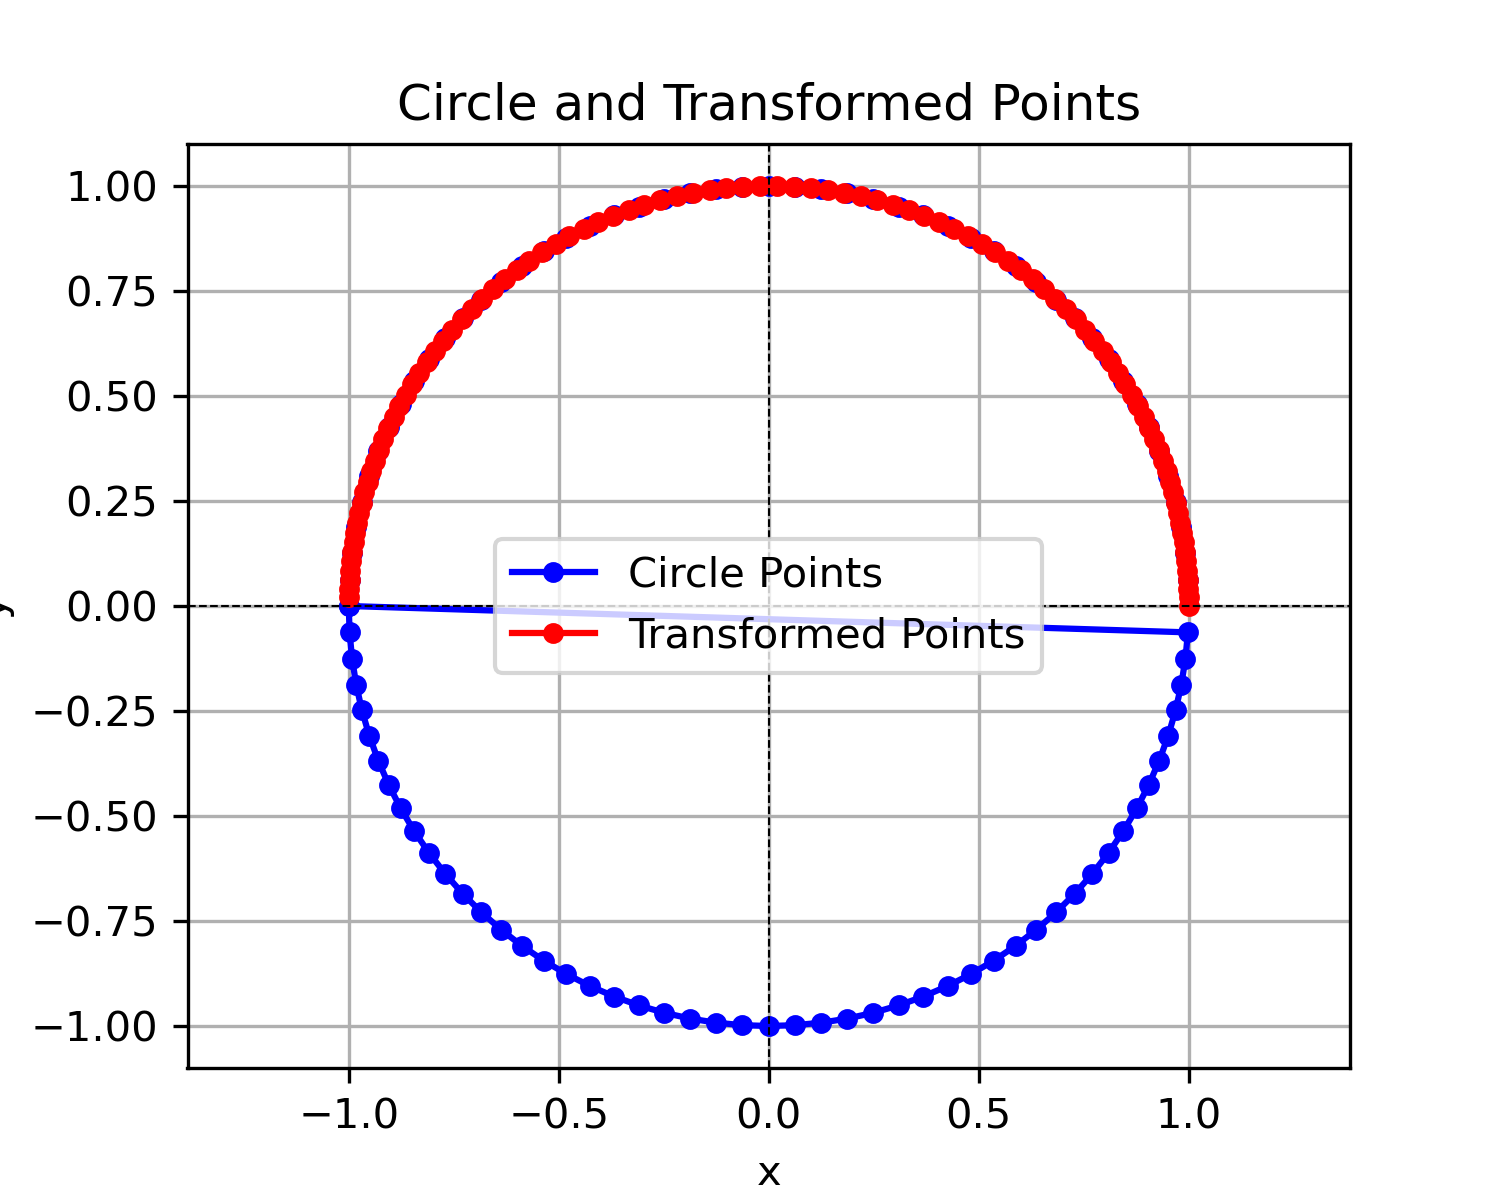
\includegraphics[width=0.8\textwidth]{figs/plot.png} 
    \caption{Circle Points}
    \label{fig:circle_plot}
\end{figure}

\end{frame}
\end{document}
